\chapter{零样本场景下基于多任务元学习的弱监督语义分割}
\section{引言}
随着遥感影像技术的快速发展,高光谱成像已成为土地资源管理中不可或缺的一个分支。
相比于多光谱成像,高光谱成像能够对同一空间区域测量数百个光谱波段,提供具有更精细波长分辨率和更丰富语义信息的连续光谱。
在过去的几十年里,高光谱成像已被应用于各种各样的领域,包括环境监测[1]、农业作物[2]、矿产地质勘探[3]、军事侦察[4]等。
\par
在高光谱成像中,光谱的丰富性使其能够准确感知和识别土地资源种类,然而这种丰富性也带来了嘈杂和不相关的噪声信息。
此外,随着维度的增加,训练一个较具鲁棒性的分类模型所需的样本量呈指数级增长,这种“维度灾难”[5]会极大影响分类模型的预测精度。
最后,数百个光谱波段也意味着需要大量的计算和存储资源,使得下游任务难以保证实时性。
因此,数据降维是消除频谱噪声、降低冗余、提高下游任务性能的必要步骤。
\par
数据降维大体可以通过两种方法来实现:特征提取和特征选择[6]。
特征提取通过应用线性或非线性变换,将原始特征空间映射到一个低维空间,生成与原始特征空间完全不同的嵌入表示。
特征选择则正如其名,从成百上千的高光谱波段中筛选出一个子集,用于代表整体的光谱信息,它消除了冗余和嘈杂的波段,而保留了最有区分度的波段[7]。
与特征提取相反,特征选择擅长于保留原始的物理信息,这使得其非常适合于真实世界场景的应用。
当特征选择应用于高光谱成像这一领域时,我们将该任务称为波段选择。
\par
在深度学习日益发展的今天,虽然高精度或高性能的波段选择算法不断涌现,仍然有一些共同问题没有被解决:
在没有考虑不同数据集间关联性的前提下,大多数现有的深度学习波段选择算法都只能处理单一特定数据集。
对于新数据集,模型参数就需要从头开始训练,这阻碍了这些算法挖掘跨不同数据集的元知识。
此外,传统全监督网络的结构通常与光谱波段数量是绑定的,而不同数据集包含不同个数的波段,这意味着同一个网络无法直接迁移到多个数据集上进行推理。
\par
高光谱图像分类 \rightarrow 语义分割
\par
零样本
\section{基于多任务元学习的高光谱图像弱监督分割框架 M$^3$GCN}
\begin{figure}[h]
\centering
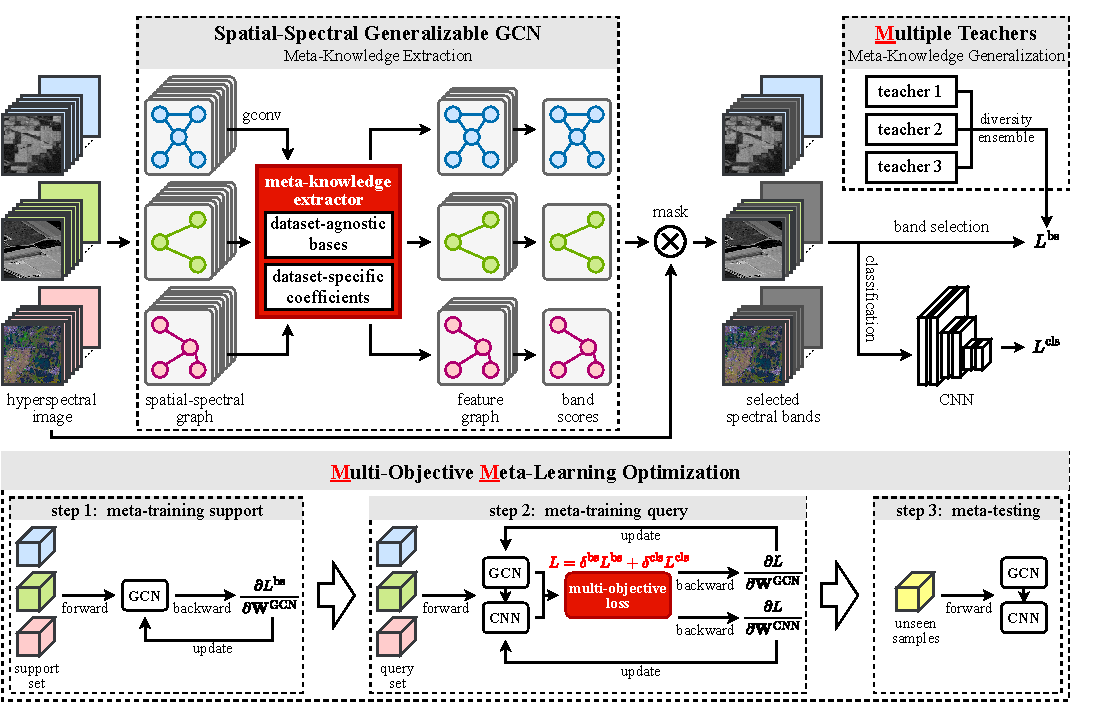
\includegraphics[width=\linewidth]{m3gcn-arch}
\caption{基于多教师多任务元学习的零样本高光谱波段选择框架 M$^3$GCN}
\label{fig:m3gcn-arch}
\end{figure}
% 空谱图
基于多教师多任务元学习的零样本高光谱波段选择框架M3GCN如图2.1所示。
首先,多个来自不同数据集的高光谱图像样本被构建为空谱图,同时考虑空间距离与谱值差异。
这些空谱图被输入到一个图卷积网络中,其可泛化的图卷积算子能够被多个波段数量不一致的数据集所共享。
这些图卷积模块的参数被进一步分解为数据集无关的基与数据集相关的系数,用于显式表征元知识。
由图卷积网络对每个波段输出得分后,选择得分高的波段作为波段选择结果,由多个预训练教师经投票融合后提供波段选择监督信息,以强化所提取到的元知识的多样性。
同时,将筛选出来的波段输入到一个卷积神经网络中执行下游分类,提供分类监督信息。
两种监督信息经多任务学习进行自动平衡,并最终结合到一个两阶段的元知识优化过程中。
\subsection{基于参数化空谱图卷积的元知识提取网络}
相比于传统的网格拓扑结构,图结构能够捕获个体间的复杂、不规则关联,这使得其非常适合于建模高光谱成像中光谱波段间的关系。
在这种建模方式下,波段及不同波段间的空间或谱间关系,将被视为图中的节点及边。
假设在我们的零样本学习场景中,共有 $\ndataset$ 个数据集 $\{ \dataset_1, \dots, \dataset_\ndataset \}$,每个数据集都包含不同数目 $\nband$ 的波段,但由这些数据集采样到的图像样本具有相同的尺寸 $\height \times \width$。
对于第 $\idataset$ 个数据集 $\dataset_\idataset$,我们所提出的光谱图可以表示为 $\graph = \{\vertset, \edgeset, \adjmat\}$。
其中,$\vertset$ 是波段节点集合,其元素 $\vertelm_{\iband} \in \vertset$ 对应第 $\iband$ 个波段;
$\edgeset$ 是波段关系边集合,其元素 $\edgeelm_{\iband,\jband} = (\vertelm_{\iband}, \vertelm_{\jband}) \in \edgeset$ 表征了第 $\iband$ 个波段和第 $\jband$ 个波段之间的联系。
\par
将单个图像样本中的所有像素一维化,就能得到第 $\iband$ 个波段的特征向量 $\ftrvec_{\iband} \in \real^{\dband}$,将所有这些特征向量堆叠起来就能得到整张图的特征矩阵 $\ftrmat \in \real^{\nband \times \dband}$。
如\figureref{fig:m3gcn-gcn}所示,特征矩阵中蓝色的行对应蓝色波段,绿色的行对应绿色波段。
图的邻接矩阵 $\adjmat \in \real^{\nband \times \nband}$ 用于描述两个节点间的相似度,被定义为空间相似度和谱间相似度的结合:
\begin{equation}
    \adjmat_{\iband,\jband} =
    \begin{cases}
        \adjmat_{\iband,\jband}^\text{spa} + \adjmat_{\iband,\jband}^\text{spec},&\text{if } \adjmat_{\iband,\jband}^\text{spa} + \adjmat_{\iband,\jband}^\text{spec} \ge \adjthres \\
        0,&\text{otherwise}
    \end{cases}
    \label{eqn:adj}
\end{equation}
\begin{equation}
    \adjmat_{\iband,\jband}^\text{spa} =
    \begin{cases}
        \exp \left( - \cfrac{1}{\nband} \vert \iband-\jband \vert \right),&\text{if } \iband \neq \jband \\
        0,&\text{otherwise}
    \end{cases}
    \label{eqn:adj-spa}
\end{equation}
\begin{equation}
    \adjmat_{\iband,\jband}^\text{spec} =
    \begin{cases}
        \exp \left( - \cfrac{1}{\dband} \Vert \ftrvec_{\iband} - \ftrvec_{\jband} \Vert_2 \right),&\text{if } \iband \neq \jband \\
        0,&\text{otherwise}
    \end{cases}
    \label{eqn:adj-spec}
\end{equation}
这里,$\adjmat^\text{spa}$ 计算第 $\iband$ 个波段和第 $\jband$ 个波段的 $1$ 维空间距离,两个波段越接近,该值就越接近 $1$;
$\adjmat^\text{spec}$ 计算特征向量 $\ftrvec_{\iband}$ 和 $\ftrvec_{\jband}$ 的 $l^2$ 欧氏距离。
同时,高斯核函数被用于将两个矩阵中数值的范围限制为 $[0,1]$。
\par
\begin{figure}[h]
\centering
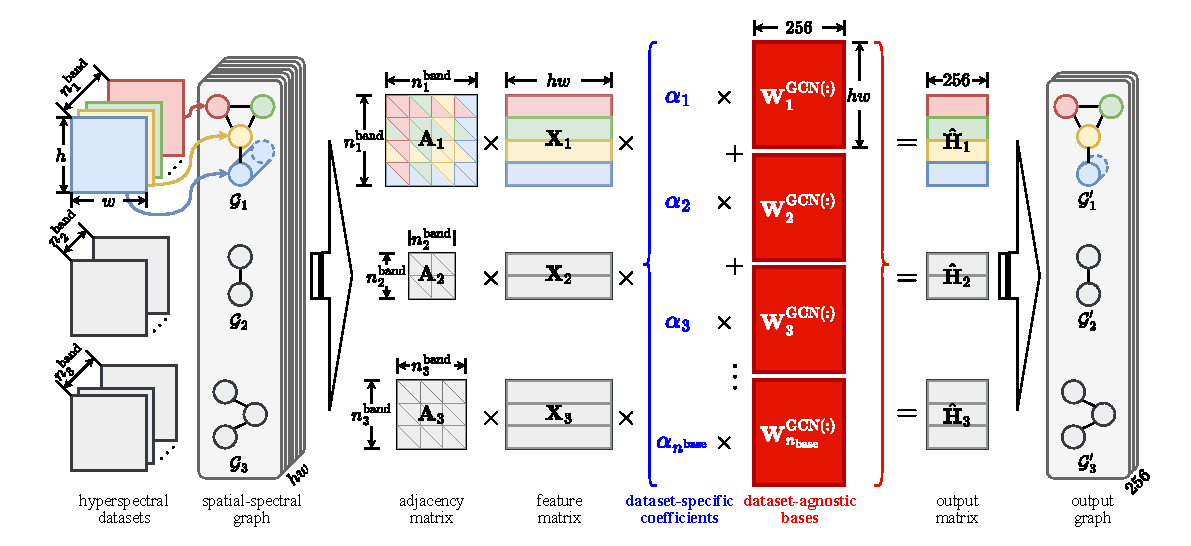
\includegraphics[width=\linewidth]{m3gcn-gcn}
\caption{参数化空谱图卷积层}
\label{fig:m3gcn-gcn}
\end{figure}
\par
% 图卷积
基于空谱波段图这一转化,我们构建了一个用于波段选择的可泛化图卷积网络[8],它由两个带有 Batch Normalization 的图卷积层所构成,第一层图卷积带 ReLU 激活函数以引入非线性,第二层图卷积带 Sigmoid 激活函数以将输出得分限定到 $[0,1]$:
\begin{equation}
    \hidmat = \relu( \bn( \widetilde{\degmat}^{-\half} \widetilde{\adjmat} \widetilde{\degmat}^{-\half} \ftrmat \wgtmat^\text{GCN(1)} ) )
    \label{eqn:gcn-gconv1}
\end{equation}
\begin{equation}
    \scrvec = \sigmoid( \bn( \widetilde{\degmat}^{-\half} \widetilde{\adjmat} \widetilde{\degmat}^{-\half} \hidmat \wgtmat^\text{GCN(2)} ) )
    \label{eqn:gcn-gconv2}
\end{equation}
其中,$\hidmat \in \real^{\nband \times \dhid}$ 表示第一层图卷积的输出特征矩阵;
$\scrvec \in [0, 1]^{\nband}$ 表示每个波段的重要性得分,用于决定选择哪些波段;
$\wgtmat^\text{GCN(1)} \in \real^{\dband \times \dhid}$ 和 $\wgtmat^\text{GCN(2)} \in \real^{\dhid}$ 是可学习参数,将在训练过程中被梯度下降所更新。
\par
% 参数化
元知识可以被理解为通过不断适应不同任务而获得的通用知识。针对元知识提取,我们提出了一种更有效的可学习参数表示方法,该方法将神经网络中的参数分解为数据集无关的基与数据集相关的系数。基充当跨数据集统一的元知识,用于同步不同数据集之间不一致的表征。系数则因其动态生成的特性而可以适应于零样本学习中未见过的新样本。具体而言,我们将图卷积核 $\wgtmat^\text{GCN(1)}$ 和 $\wgtmat^\text{GCN(2)}$ 参数化为基的线性组合:
\begin{equation}
    \wgtmat^\text{GCN(:)} = \alpha_1\wgtmat_1^\text{GCN(:)} + \dots + \alpha_{n^\text{base}}\wgtmat_\nbase^\text{GCN(:)}
    \label{eqn:gcn-condconv}
\end{equation}
其中 $\wgtmat_1^\text{GCN(:)} \dots \wgtmat_\nbase^\text{GCN(:)}$ 是正交基,$\alpha_1 \cdots \alpha_\nbase$ 是线性组合中的系数,这些系数是由一个平均池化层、一个全连接层及一个 Sigmoid 激活函数所输出的:
\begin{equation}
    \alpha_1 \dots \alpha_\nbase = \sigmoid( \frac{1}{\nband} \mathbf{1}^\top \ftrmat \wgtmat^\text{FC} )
    \label{eqn:gcn-condconv-alpha}
\end{equation}
这里 $\frac{1}{\nband} \mathbf{1}^\top \in \real^{1 \times \nband}$ 沿着特征矩阵 $\ftrmat$ 的每一列计算均值,$\wgtmat^\text{FC} \in \real^{\height\width \times \nbase}$ 将池化后的特征矩阵映射为 $\nbase$ 个标量,对应 $\nbase$ 个参数基。
据此,元知识就被显式表示为了这些数据集无关的基,而那些数据集相关的系数就可以用于刻画各数据集独有的特征了。
% 波段选择
对所有波段都计算得分,形成分数向量 $\scrvec$ 后,就可以决定要选择的波段子集了。
通常情况下,我们需要提前确定好超参数 $\nsband$,作为要选择的波段数量($\nsband < \nband$)[9]。
为了使波段选择的输出能够作为下游分类任务的输入,我们使用二值化算子将分数向量转换为一张波段掩码图:
\begin{equation}
    \scrthres = \left\{ \scrvec_{o_1}, \scrvec_{o_2}, \cdots, \scrvec_{o_\nband} \right\}_{\nsband}
    \label{eqn:threshold}
\end{equation}
\begin{equation}
    \mskvec
    = \bin(\scrvec, \scrthres)
    =
    \begin{cases}
        0,&\text{if } \scrvec_{\iband} \geq \scrthres \\
        1,&\text{otherwise}
    \end{cases}
    \label{eqn:binarization}
\end{equation}
\par
执行波段选择的流程如下:
首先,所有波段的得分都按降序排列成 $o_1, o_2, \cdots, o_{\nband}$,此时阈值 $\scrthres$ 就是排序后的第 $\nsband$ 个分数;
接着,二值化算子 $\bin(\cdot)$ 将波段序列转换为一张波段掩码图 $\mskvec \in \{0,1\}^{\nband}$,其值仅在波段分数大于阈值时才设置为 $1$;
最后,该波段掩码图被乘到输入的高光谱图像上,作为后续分类网络的输入。
\subsection{基于多教师投票融合的元知识强化模块}
作为下游任务的一种典型的预处理过程,波段选择不像其他全监督任务(例如图像分类)那样具有监督标签,它通常被形式化为一种无监督任务[10],或者是借助于辅助的分类器进行性能评估[11]。
基于这种训练方式的波段选择算法要么精度较差,要么需要消耗大量的训练时间。
此外,这些算法也无法推广到未见过的新样本上,导致零样本波段选择不可行。
因此,除了分类损失,我们还利用了来自多个波段选择教师的高质量监督,构建了辅助损失函数。
这种额外监督不仅提升了第2.1节中元知识的泛化性和适应性,还加速了模型收敛过程,减少了训练时间的消耗。
\par
具体来说,我们首先挑选了三个分别基于滤波、基于封装、基于嵌入的算法作为教师并进行预训练,以便提前准备好高质量的监督来源。
考虑到在多个教师之间实现平衡,我们制定了一种多教师投票融合策略用于多样性集成,该策略能够根据每个波段得到的票数来选择波段子集。
在这些教师分别选择各自的波段子集之后,我们定义一个计数函数 $\text{cnt}(i)$ 来表示第 $\iband$ 个波段收到的票数。
最后,根据计数函数的值对波段进行降序排列,就可以选择其中得票最多的波段作为结果了:
\begin{equation}
    \mathbb{S} = \left\{ \underbrace{i_1, \dots}_{\text{cnt}(i) = 3} \underbrace{i_7, i_8, \dots \dots}_{\text{cnt}(i) = 2} \underbrace{i_{22}, i_{23}, \dots \dots \dots}_{\text{cnt}(i) = 1} \right\} _{1, \dots, \nsband}
    \label{eqn:divens-set}
\end{equation}
\begin{equation}
    \bsgtvec_i =
    \begin{cases}
        1,&\text{if } i \in \mathbb{S} \\
        0,&\text{otherwise}
    \end{cases}
    \label{eqn:divens}
\end{equation}
这里,$\bsgtvec$ 表示用于直接监督波段选择任务的标签。
为了公平起见,对于那些票数相同的波段,我们随机选择一个波段数量合适的子集作为结果。
通过这种融合策略,多个教师可以被集成为一个更强大的教师。
不同教师的不同优化方向能够有效缓解多样性的缺失,进而更好地泛化到零样本学习中的新样本上。
最终,波段选择损失被定义为图卷积网络预测的波段分数与集成教师输出的离散波段间的多标签二元交叉熵损失:
\begin{equation}
    \loss^\text{bs} = \bsgtvec \log\scrvec + (\mathbf{1} - \bsgtvec) \log( \mathbf{1} - \scrvec )
    \label{eqn:loss-bs}
\end{equation}
\subsection{基于多任务学习的多目标自动平衡损失}
分类损失和波段选择损失都对我们的任务有帮助,这启示我们,可以使用一个集成的损失函数同时对二者进行优化。
直观来看,要合并多个损失函数,可以简单地通过加权求和的形式来实现:
\begin{equation}
    \loss = \weight^\text{bs} \loss^{\text{bs}} + \weight^\text{cls} \loss^{\text{cls}}
    \label{eqn:loss}
\end{equation}
其中,$\weight^\text{bs} \in [0,1]$ 和 $\weight^\text{cls} \in [0,1]$ 分别是波段选择损失和分类损失的相对权重。
对于 $\ndataset$ 个不同的高光谱数据集,总共有 $2\ndataset$ 个这样的超参数 $\{ \weight_1^\text{cls}, \dots, \weight_\ndataset^\text{cls}, \weight_1^\text{bs}, \dots, \weight_\ndataset^\text{bs} \}$ 需要人工调优。
事实上,波段选择任务的最终精度很大程度上取决于这些相对权重的设置[12],而这些权重的人工调优需要耗费大量的实验成本。
\par
更理想的方式是让这些权重能够随着网络训练而自动被学习到。
受[13]的启发,我们提出了一种多任务学习方法,该方法根据任务的不确定性对多个损失函数进行自动加权。
[13]中说明,模型输出和样本标签之间的偶然误差可以被建模为一种不确定性,进而允许我们将多任务损失分解为多个似然的乘积。
通过分别将波段选择任务和分类任务估计为 Sigmoid 似然与 Softmax 似然,我们可以定义如下的多目标平衡损失:
\begin{equation}
\begin{split}
\loss
&= -\log \sigma(\scrvec_\idataset;\ \wgtmat^\text{GCN}, \weight^\text{bs}) \nonumber\\
&\qquad\qquad \cdot \softmax(\prbvec_\idataset;\ \wgtmat^\text{GCN}, \wgtmat_\idataset^\text{CNN}, \weight^\text{cls}) \nonumber\\
&\propto \weight^\text{bs} \loss^\text{bs} + \weight^\text{cls} \loss^\text{cls} + \log\sqrt{\frac{1}{\weight^\text{bs}}} + \log\sqrt{\frac{1}{\weight^\text{cls}}} 
\end{split}
\label{eqn:loss-uncertainty}
\end{equation}
其中,$\weight^\text{bs}$ 和 $\weight^\text{cls}$ 分别是两个目标的权重。
受限于正则项 $\log\sqrt{1 / {\weight^\text{bs}}}$ 和 $\log\sqrt{1 / {\weight^\text{cls}}}$ 的存在,这些权重不至于变得过小。
通过应用此多目标损失,目标的权重能够通过梯度下降而自动被学习到,无需任何人工调优,从而大幅减少了超参数调优成本。
同时,目标的权重能够在模型训练过程中被动态地更新,进而自动适应于不同的训练阶段。
\subsection{基于两阶段元学习的元知识优化流程}

\floatname{algorithm}{\textbf{算法}}
\renewcommand{\algorithmicrequire}{\textbf{输入:}}
\renewcommand{\algorithmicensure}{\textbf{输出:}}
\begin{algorithm}
\begin{algorithmic}
\Require
元训练任务 $\mathcal{D}_1^\text{train}, \dots, \mathcal{D}_{n^\text{ds}}^\text{train}$,
元测试任务 $\mathcal{D}^\text{test}$,
学习率 $\alpha$,
元学习率 $\beta$,
训练轮数 $T$
\Ensure
训练好的网络参数 $\mathbf{W}^\text{GCN(:)}, \mathbf{W}^\text{CNN}_1, \dots, \mathbf{W}^\text{CNN}_{n^\text{ds}}$
\State 初始化相对权重:$\lambda^\text{bs}\vert_{t=1} \leftarrow 1, \lambda^\text{cls}\vert_{t=1} \leftarrow 1$
\For {训练轮次 $t = 1, \dots, T$}
    \For {$\{\mathcal{D}^\text{train}_1, \dots, \mathcal{D}^\text{train}_{n^\text{ds}}\}$ 中的每个元训练任务 $\mathcal{D}^\text{train}_k$}
        \State 将样本分为支撑集和查询集:$\mathcal{D}_k \rightarrow \{ \mathcal{D}^\text{spt}_k, \mathcal{D}^\text{qry}_k \}$ % Spilt into a support set and a query set by the ratio of 3:7
        \State 复制一份参数:$\mathbf{W}^\text{GCN}_k \leftarrow \mathbf{W}^\text{GCN}$ % Synchronize parameters among GCNs
        \For {支撑集 $\mathcal{D}^\text{spt}_k$ 中的每个批次}
            \State 将所有像素一维化成特征矩阵 $\mathbf{X}$
            \State 构建邻接矩阵 $\mathbf{A}$
            \State 构建空谱图 $\mathcal{G} = \{ v, \mathcal{E}, \mathbf{A} \}$
            \State 通过 $\mathbf{W}^\text{GCN}$ 推理得到 $\hat{\mathbf{s}}$ 
            \State 使用预训练教师投票得到 $\mathbf{s}$
            \State 评估波段选择损失 $\mathcal{L}^\text{bs}$
            \State 回传梯度,计算 $\partial{\mathcal{L}^\text{bs}}/\partial{\mathbf{W}_k^\text{GCN}}$
            \State 使用梯度下降更新 $\mathbf{W}^\text{GCN}_k$:\\
            $\mathbf{W}^\text{GCN}_k\vert_{t+1} = \mathbf{W}^\text{GCN}_k\vert_t + \alpha \cdot \partial{\mathcal{L}^\text{bs}}/\partial{\mathbf{W}^\text{GCN}_k\vert_t}$
        \EndFor
        \For {查询集 $\mathcal{D}^\text{qry}_k$ 中的每个批次}
            \State 仿照上述步骤计算得到 $\hat{\mathbf{s}}$ 和 $\mathcal{L}^\text{bs}$
            \State 将 $\hat{\mathbf{s}}$ 二值化成为掩码图 $\hat{\mathbf{M}}$
            \For {当前批次中的每个图像 $x_i$ 和它的类别标签 $y_i$}
                \State 通过逐元素乘法,使用 $\hat{\mathbf{M}}$ 对 $x_i$ 进行选择:$x_i \leftarrow x_i \cdot \hat{\mathbf{M}}$
                \State 将 $x_i$ 通过 $\mathbf{W}^\text{CNN}_k$ 推理,得到一个概率向量 $\hat{\mathbf{y}}_i$
            \EndFor
            \State 评估分类损失 $\mathcal{L}^\text{cls}$
            \State 评估多目标平衡损失 $\mathcal{L}$
            \State 回传梯度以计算 $\partial{\mathcal{L}}/\partial\lambda^\text{bs}$、$\partial{\mathcal{L}}/\partial\lambda^\text{cls}$、$\partial{\mathcal{L}}/\partial{\mathbf{W}^\text{GCN}_k}$ 和 $\partial{\mathcal{L}}/\partial{\mathbf{W}^\text{CNN}_k}$
            \State 为 $\mathbf{W}_k^\text{GCN}$ 累积梯度 $\partial{\mathcal{L}}/\partial{\mathbf{W}^\text{GCN}_k}$
            \State 使用梯度下降更新 $\lambda^\text{bs}$、$\lambda^\text{cls}$ 和 $\mathbf{W}_k^\text{CNN}$:\\
            $\lambda^\text{bs}\vert_{t+1} = \lambda^\text{bs}\vert_t + \alpha \cdot \partial{\mathcal{L}}/\partial{\lambda^\text{bs}\vert_t}$\\
            $\lambda^\text{cls}\vert_{t+1} = \lambda^\text{cls}\vert_t + \alpha \cdot \partial{\mathcal{L}}/\partial{\lambda^\text{cls}\vert_t}$\\
            $\mathbf{W}^\text{CNN}_k\vert_{t+1} = \mathbf{W}^\text{CNN}_k\vert_t + \alpha \cdot \partial{\mathcal{L}}/\partial{\mathbf{W}^\text{CNN}_k\vert_t}$
        \EndFor
        \State 为 $\mathbf{W}_k^\text{GCN}$,沿着所有批次计算 $\partial{\mathcal{L}}/\partial{\mathbf{W}^\text{GCN}_k}$ 的均值
        \State 为 $\mathbf{W}^\text{GCN}$,将 $\partial{\mathcal{L}}/\partial{\mathbf{W}^\text{GCN}_k}$ 累加到 $\partial{\mathcal{L}}/\partial{\mathbf{W}^\text{GCN}}$:\\
        $\partial{\mathcal{L}}/\partial{\mathbf{W}^\text{GCN}} \leftarrow \partial{\mathcal{L}}/\partial{\mathbf{W}^\text{GCN}} + \partial{\mathcal{L}}/\partial{\mathbf{W}^\text{GCN}_k}$
    \EndFor
    \State 通过梯度下降更新 $\mathbf{W}^\text{GCN}$,以用于元学习:\\
    $\mathbf{W}^\text{GCN}\vert_{t+1} = \mathbf{W}^\text{GCN}\vert_t + \beta \cdot \partial{\mathcal{L}}/\partial{\mathbf{W}^\text{GCN}}$
\EndFor
\end{algorithmic}
\caption{M$^3$BS 的两阶段元学习优化过程}
\label{alg3}
\end{algorithm}

\section{实验结果与分析}
\subsection{高光谱图像语义分割数据集}
\subsection{与其他语义分割算法的比较}
\subsection{针对 M$^3$GCN 的消融实验}
\subsection{针对 M$^3$GCN 的超参数敏感性分析}
\section{本章小结}
